% Created 2019-06-10 Mon 00:29
% Intended LaTeX compiler: pdflatex
\documentclass[a4paper]{article}
\usepackage[utf8]{inputenc}
\usepackage[T1]{fontenc}
\usepackage{graphicx}
\usepackage{grffile}
\usepackage{longtable}
\usepackage{wrapfig}
\usepackage{rotating}
\usepackage[normalem]{ulem}
\usepackage{amsmath}
\usepackage{textcomp}
\usepackage{amssymb}
\usepackage{capt-of}
\usepackage{hyperref}
\usepackage{amsmath,amssymb}
\usepackage{empheq}
\usepackage{float}
\author{Marcelo Finger, Thiago Lira}
\date{May 28, 2019}
\title{Using Deep Learning Bayesian Methods do Predict Cement Compressive Strength with Uncertainty}
\hypersetup{
 pdfauthor={Marcelo Finger, Thiago Lira},
 pdftitle={Using Deep Learning Bayesian Methods do Predict Cement Compressive Strength with Uncertainty},
 pdfkeywords={},
 pdfsubject={},
 pdfcreator={Emacs 26.1 (Org mode 9.2.1)}, 
 pdflang={English}}
\begin{document}

\maketitle
\begin{abstract}
Prediction of cement compressive strength (CCS) is an im-
portant step in quality assurance in the industrial production
of construction materials. The literature has recognized that
laboratory data provides a limited analysis on isolated sam-
ples, and recent work on predicting CCS considers cement
data time-series obtained on factory floor. This works extends
this approach, providing Bayesian Deep Learning techniques
to generate machine learning models to support decision mak-
ing activities aiming at the stability of the industrial process
in the presence of uncertainty. These models are able to scale
to huge amounts of data, require no specific knowledge of the
data and provide powerful uncertainty estimates, which are
updated in a day-to-day basis incorporating new data pro-
duced on the factory.
\end{abstract}


\section{Introduction}
\label{sec:org605e643}
The prediction of the compressive strength of cement (CCS) has been recognized of great importance to the civil construction industry, 
given that this capacity is one of the factors to assess the quality of cement \cite{cementnn0}.

The 28-day compressive strength (RC28) is chosen as the measurement used as a regulatory parameter in construction codes, and the variance of these measurements can 
indicate the stability of the industrial process. 

It is important for the industry to have a system that, detecting drops on the quality of the cement, can point to anomalies on the process (e.g. concentration of reagents) 
probably causing it. The problem can them be tackled with supervised learning \cite{dlbook}, where the target are the RC28 measurements and the inputs are chemical compositions and other 
quantities measured on a daily basis on the factory.

Past work \cite{cementlin,nncement} on the problem focused on laboratorial analyses. We extend this approach to account for the dynamical nature of the industrial process, providing 
an analysis that can be made on a daily basis on the industrial floor, as is done in \cite{dynstat}.

Past work on this more industry-aware front \cite{greciaLin} makes the distinction between dynamic and static models to predict the CCS. 
The authors propose a dynamic moving window linear regression that recalculates it's regression parameters every time a new RC28 measurement is ready. 
This dynamical model is also able to provide standard deviations for the regression parameters.

Following that idea, we shall consider all the cement data as time series (i.e. indexed by time), 
with the assumption that the past of the measurements have some information concerning the future of the process.
Our data was provided by brazilian's cement company Intercement.   

For many decades the state-of-the-art on forecasting has been the ARIMA class of models, and Box-Jenkins procedures \cite{inbook}, but these models have their limitations. 
They are unable to model non-linear relationships on the data \cite{forecasting}, and many real world processes happen to be non-linear. These models also have trouble using exogenous variables 
to aid the time series forecasting \cite{ubertime}.

Recently many time series problems on different domains had it's classical results beaten by new Deep Learning methods such as Recurrent Neural Network models \cite{energylstm,lstmbr},
these deep learning models require no \emph{feature engineering} (i.e. specific knowledge about the data) and work very well even with gigabytes of data \cite{ARIMA_LSTM}. 
They are more data-driven than classical methods that assume very little about the data, meaning that little manual tweaking on the model parameters is necessary.

Classic time series models fail to scale well to huge amounts of data, although they are able to provide good uncertainty estimates \cite{deepar}. Past work \cite{DIAZROBLES20088331,KHASHEI2010479} 
has managed to combine ARIMA models with Artificial Neural Networks (ANN), with better results than just either of these models.

We then use a new approach, implementing Bayesian Deep Learning techniques to leverage the scalability of Deep Learning with the uncertainty estimation of Bayesian Statistics. 
This last feature is particularly useful on a industrial setting, as to provide decision making evidence on the factory floor \cite{deepfactors}. 

\subsection{Objectives}
\label{sec:org516287e}

We shall bring these new Bayesian Deep Learning techniques to the CCS prediction domain. The contributions of this paper are 
as follows: 

\begin{itemize}
\item A comparison of 3 state-of-the-art Bayesian Deep Learning models for time series forecasting on a new domain for these techniques.
\end{itemize}

\subsection{Paper Structure}
\label{sec:org4637cc7}
The rest of the paper is organized as follows:  Section \ref{sec:org043fe2d} gives a brief overview of each model used and a formal definition of the supervised learning problem; Section \ref{sec:orge452161} specifies how the data was transformed and treated before 
used on the learning task; Section \ref{sec:orge2fc0dd} details our experiments and results with the models; Section \ref{sec:org1323f05} gives a final word and future directions of research. 
\section{Preliminaries}
\label{sec:org043fe2d}

The training data is composed of the pairs \((\{\textbf{x}_{t_0},y_{t_o}\},\{\textbf{x}_{t_1},y_{t_1}\}, \dots, \{\textbf{x}_{T},y_{T}\})\) on the time span \([t_o,T]\). 
Let F be a finite time horizon, such that F > T, the models should learn a probability distribution of the form:

\begin{equation}
p(y_{T:F} | y_{t_{o}:T},\textbf{x}_{t_{0}:T}) 
\end{equation} 

Meaning that we want to model the distribution of the next (\(F-T\)) \(y\) values, given some past horizon of \(x\) and \(y\) values. Contextualized on our data, the targets \(y_t\)
are the RC28 measurements and \(x_t\) are the covariates (i.e. exogenous variables), specified on Section \ref{sec:orge452161}.

We now shall briefly explain each model used:

\subsection{Deep Factors \cite{deepfactors}}
\label{sec:org7cac535}

The Deep Factors Model combines a LSTM time series regression model to model the "global" part of the predictions, and a Gaussian Process to model the "local" part
i.e. the noise and uncertainty. 

\subsubsection{Gaussian Process}
\label{sec:org41b8df1}
A Gaussian Process \cite{gpml} is a collection of random variables, such that every linear combination of them are normally distributed. The process is completely specified by it's
mean function and a covariance function, or kernel. 

\[
f(x) \sim \mathcal{GP}( m(x), K(x,x'))
\]

The most common kernel used for regression tasks is the exponential kernel, it captures the distance between variables in 
the euclidean sense.

\[
  K(x,x') = \exp(-\frac{1}{2}|x - x'|^2)
\]

\subsubsection{Generative Model}
\label{sec:orgaa53833}
An observed value from the Deep Factors model \(y^*_{i,t}\) is the sum of the weighted average on the global parts learned by the LSTM cell and the local flutuaction
given by the Gaussian Process:

\[
  \textbf{Local effect: }  r_i \sim \mathcal{GP} (0, K_i(.,.))
\]

\[
  \textbf{Fixed effect:}  f_{i,t} = W_ig_t(x_{i,t})
\]

These effects are combined via a latent function \(u_{i,t}\), to form the generative model: 

\[
  \textbf{Emission: }  y^*_{i,t} \sim p(. | u_{i,t}) , u_{i,t} = r_{i,t} + f_{i,t}  
\]

The model is optimized by maximizing the marginal likelihood of the predictions, in a similar fashion to the other models presented in this work. 
In this case, \(p(.|u_{i,t})\) is Gaussian, so the marginal likelihood can be computed easily, where \(\sigma_i\) is an additional parameter to stabilize the covariance:

\[
p(y^*_{i}) = \mathcal{N}(f_i,K_i + \sigma_i^2\mathcal{I})
\]

\subsection{DeepAR \cite{deepar}}
\label{sec:org5bcf060}

This model uses an autoregressive RNN architecture to model the probability distribution of predictions on a forecast horizon of a time series. The likelihood function can be choosen given the statistical
characteristics of the problem. For this problem we use a Gaussian Likelihood.

The model is described via the following autoregressive equation, the \(y_{i,t}\) term is the real value of the previous timestep annotation (the autoregressive term), as we are in the training regime:

\begin{center}
\(h_{i,t} = h(h_{i,t-1},y_{i,t-1},x_{i,t}, \theta)\)
\end{center}
The hidden state \textbf{\textbf{h}} of a timestep is then used to calculate the mean 
and standard deviation of it's prediction:

\begin{center}
\(\mu(h_{i,t}) = W_{\mu}h_{i,t} + b_{\mu}\) 

\(\sigma(h_{i,t}) = \log(1 + \exp(W_{\sigma}h_{i,t}+ b_{\sigma}))\) 
\end{center}
It is then a simple matter of using a Gaussian Marginal Likelihood with parameters \(\mu\) and \(\sigma\) to 
calculate the model's cost function and propagate it's error.

For making predictions, we use a Monte Carlo trace. Each timestep's output is a \textbf{\textbf{distribution}} parametrized by \(\mu\) and \(\sigma\), which enables us to make quantile forecasts for each timestep.
The autoregressive term for the next timestep is just a sample from the last timestep's distribution.

\[ y^*_{i,t-1}  \sim \mathcal{N}(\mu(h_{i,t}),\sigma(h_{i,t})) \]



\subsection{Encoder Decoder Forecaster \cite{ubertime}}
\label{sec:org6cbdba3}
This model proposed by Uber implements a Bayesian Neural Network (BNN) via the Monte Carlo Dropout technique (a variational inference aproximation),
which them enables the model to decompose it's prediction uncertainty into three types:
model uncertainty, inherent noise and model misspecification. We assume a Gaussian Likelihood as
our data generating distribution: 

\begin{equation}
y| \theta \sim \mathcal{N}(y;f^{\theta}(x),\,\sigma^2)
\end{equation}

Following the Bayesian aproach, we would integrate over the distribution of
our model parameters \(\theta\), to get to the distribution of the predictions given new inputs 
p(y\textsuperscript{*} | x\textsuperscript{*}). The variance of this distribution can be calculated via the Law of Total Variance:

\begin{equation}
Var[y^* | x^*] = Var[f^{\theta}(x^*)] + \sigma^2  
\end{equation}

Where \(\sigma\) (the inherent noise) is estimated using the validation data and Var[f\textsuperscript{W}(x\textsuperscript{*})] (the model uncertainty)
is given by the Monte Carlo Dropout Technique. This value is estimated via the sample variance 
of \textbf{\textbf{B}} stochastic realizations of a prediction, using the trained model: 

\begin{equation}
Var[f^{\theta}(x^*)]  = \frac{1}{B}\sum^B_{B=1}(\hat{y}^*_{(B)} - \hat{y}^*)^2  
\end{equation}

\section{Methodology}
\label{sec:orge452161}

We shall evaluate the performance of 3 Bayesian Deep Learning models on the 28-day CCS prediction learning task. The raw data is first preprocessed 
before it can be used on a time-series forecasting setting. This process is explained next:

\subsection{Data}
\label{sec:org75a0797}

The data represents 11 years of cement production on a medium sized factory, located on the city of Cajati.  

For the models, we use the data from the last phase of the production of cement. The measurements represent the cement when it is ready to be shipped. 
On this particular dataset, we have 2408 almost daily annotations spanning 11 years of cement production, with 25 collums (i.e. features) per day.

From this data, we remove the columns of measurements that had a frequency too little to be of use statistically (i.e. < 70\% of all days with data).

The data is first resampled (and filled with the mean in the case of missing values) so that we don't have any days without measurements. 
Since we are dealing with inputs of different orders of magnitude, we first rescale the data to be in the [0,1] range with the minmax method. Let  \(\textbf{x}\) be a column of data, it's 
normalized value \(\textbf{z}\) will be:


\begin{equation}
z=\frac{x-\min (x)}{\max (x)-\min (x)}
\end{equation}

After cleaning, the columns with enough data to be useful at the learning task are: 

\begin{itemize}
\item (i) Percentages related to chemical composition: AL\textsubscript{2}O\textsubscript{3}, SIO\textsubscript{2}, MGO, RICARB, P\textsubscript{2}O\textsubscript{5} and FE\textsubscript{2}O\textsubscript{3}
\item (ii) Percentage of the matter of water relative to the cement: AGP
\item (iii) Time (in seconds) that the material takes to begin hardening and to finish hardening, respectively: IP, FP
\item (iv) Blaine fineness, measured in square centimeters per gram: SBL
\item (v) Percentage of Mass lost on furnace: FP
\item (vi) The CCS measurements made after 3, 7 and 28 (our target) days of expedition of that particular sample: RC3, RC7, RC28
\end{itemize}


Using the Machine Learning approach \cite{dlbook},  we shall let the model learn by itself what parameters to give more importance, 
thus not doing any \emph{feature engineering} prior to training the model, i.e. we shall not 
use any civil engineering or chemistry knowledge to alter the models or the data in any way.

\subsection{RC3, RC7 and RC28}
\label{sec:orgfbd87b6}
Every day \(t\) a new lot of cement is ready and expedited from the factory. This lot doesn't have RC3, RC7 or RC28 measurements yet made. The task is to predict with a margin of confidence 
the RC28 value of this specific lot. From this lot we have multiple concentrations and quantities of reagents annotated from the factory as inputs.

Following the methodology of \cite{greciaLin}, we will have the RC3 and RC7 measurements along with the other inputs. But if we are predicting the compressive strength of day \(t\), the RC3 and RC7 measurements
will come from the last lots of cement of which this measurement is available on that day i.e. from the lots of the days \(t-3\) and \(t-7\) respectively. This is to ensure that such analysis
can be done with new day, on the day of it's expedition, thus not confining our analysis just to older samples i.e. ones from which we already know it's RC3, RC7 and RC28 measurements. 

\subsection{Train/Test Separation}
\label{sec:orgb00d5fa}
We shall use data from 01/2007 to 09/2018 as our training data, and the last 3 months of 2018 (where our data ends) as our validation data, as we are assuming that the past of the process
can give information about it's future.

We shall then evaluate how long in the future can the models reliably predict new measures with an acceptable uncertainty.
It's expected that the validation error will increase the farther we try to predict the RC28 measure on the future.

\section{Experiments}
\label{sec:orge2fc0dd}

All models were implemented using PyTorch \cite{pytorch}, for the Gaussian Processes we use GPyTorch \cite{gpytorch}. The hyperparameters chosen for each model are shown on Table [?]. 

Every RNN based model will have a certain window of data as input to predict the next day of RC28. The size of this window is fixed across models so that we might compare it's accuracies. 

The models forecast performance will be evaluated by two metrics: One of which, the Quantile Loss (or \(\rho\)-risk), will assess the quality of the uncertainty measure,
and the RMSE will assess the error. 

Given a true value y\textsubscript{t} and a quantile prediction y\textsuperscript{*}\textsubscript{t}(\(\rho\)), with  1 > \(\rho\) > 0. The Quantile Loss is defined as:


\begin{equation*}
  \mathcal{QL}_{\rho}(y_{t},y^{*}_{t}(\rho)) =
\begin{cases}
  2 \rho(y_{t} - y^{*}_{t}(\rho)) & \text{if }  y_{t} - y^{*}_{t}(\rho) > 0 \\
  2 (1 - \rho)(y^{*}_{t}(\rho) - y_{t}) & \text{if } y_{t} - y^{*}_{t}(\rho) \leq 0
\end{cases}
\end{equation*}

To compare the models we shall use the normalized sum of quantile losses, or \(\rho\)-risk. 

\begin{equation*}
\sum_{t}\frac{\mathcal{QL}_{\rho}(y_{t},y^{*}_{t})}{\sum_{t}y_{t}}
\end{equation*}

We will use the values of \(\rho\) 0.5 and 0.9. These values can be understood as the expected error on 50\% and 90\% of the sampled values, respectively. 
The .5-risk is equivalent to the mean absolute percentage error (MAPE).


The RMSE loss for a predicted time series \(\mathbf{y^*}\) and it's true values \(\mathbf{y}\) is defined as:

\begin{equation*}
RMSE(\mathbf{y}^*,\mathbf{y}) = \sum^n_{t}\sqrt{\frac{(y_t - y^*_{t})^2}{n}}
\end{equation*}


\subsection{Results}
\label{sec:orgaf686f1}

Table \ref{tab:org419d531} reports how each model performs as a function of the timespan of forecasting. 
The error increases as time passes, as is expected. All models perform well on the 24h (next-day) forecasting.

\begin{center}
\begin{table}[htbp]
\caption{\label{tab:org419d531}
RMSE values by forecast span}
\centering
\begin{tabular}{rr}
\hline
Deep Factors & RMSE\\
\hline
24h & 0.18\\
3d & 2.36\\
7d & 1.83\\
\hline
Deep AR & RMSE\\
\hline
24h & 0.07\\
3d & 1.37\\
7d & 1.44\\
\hline
Encoder Decoder & RMSE\\
\hline
24h & 0.22\\
3d & 0.36\\
7d & 1.04\\
\hline
\end{tabular}
\end{table}
\end{center}

Next, Figures \ref{fig:orgbc84a58}, \ref{fig:org32bded3} and \ref{fig:org484f42d} report the full prediction on the dev set timespan, with it's uncertainties.

\begin{figure}[H]
\centering
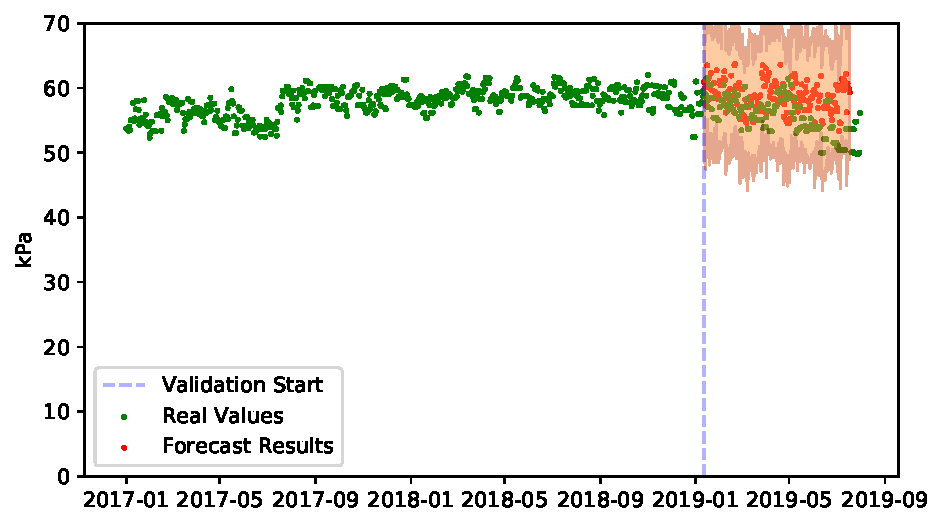
\includegraphics[height=0.3\textwidth]{/Users/thiagolira/Dropbox/Mestrado/Intercement/paper_img/forecast_enc_dec.pdf}
\caption{\label{fig:orgbc84a58}
Forecast Results for Encoder Decoder Model}
\end{figure} 

\begin{figure}[H]
\centering
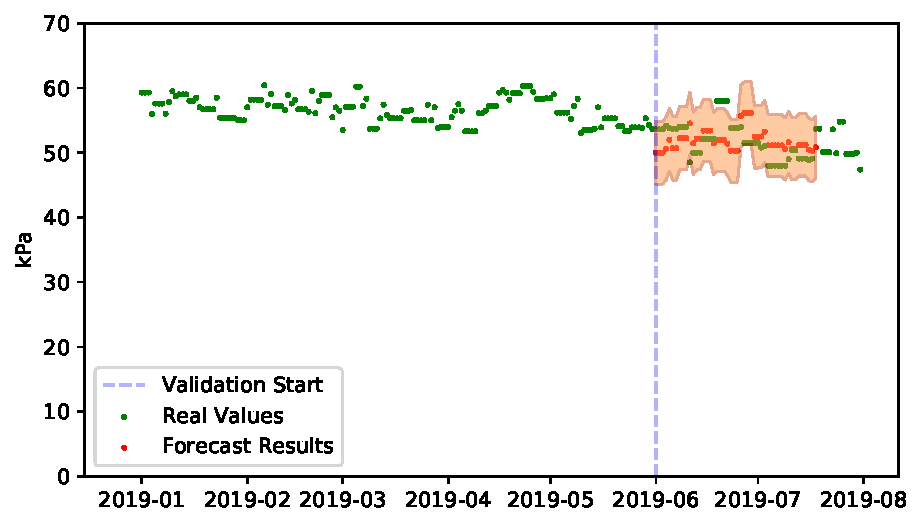
\includegraphics[height=0.3\textwidth]{/Users/thiagolira/Dropbox/Mestrado/Intercement/paper_img/forecast_deep_factors.pdf}
\caption{\label{fig:org32bded3}
Forecast Results for Deep Factors Model}
\end{figure} 

\begin{figure}[htbp]
\centering
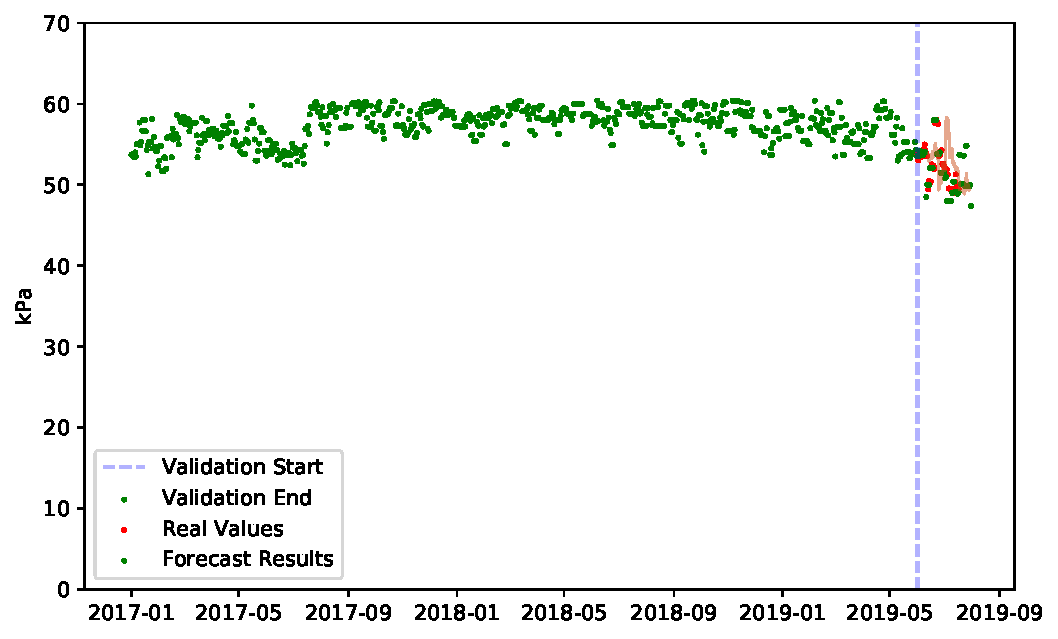
\includegraphics[height=0.3\textwidth]{/Users/thiagolira/Dropbox/Mestrado/Intercement/paper_img/forecast_deep_ar.pdf}
\caption{\label{fig:org484f42d}
Forecast Results for Deep AR Model}
\end{figure} 

We now plot the predictions for 90 days after T of the models against it's true values, to evaluate the distribution of the predicted values.

\begin{center}
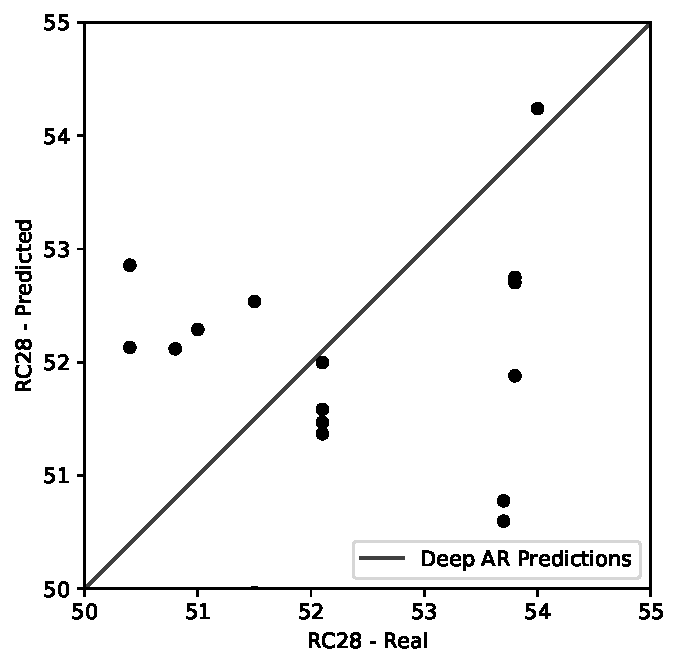
\includegraphics[height=0.3\textwidth]{/Users/thiagolira/Dropbox/Mestrado/Intercement/paper_img/qq_deep_ar.pdf} 
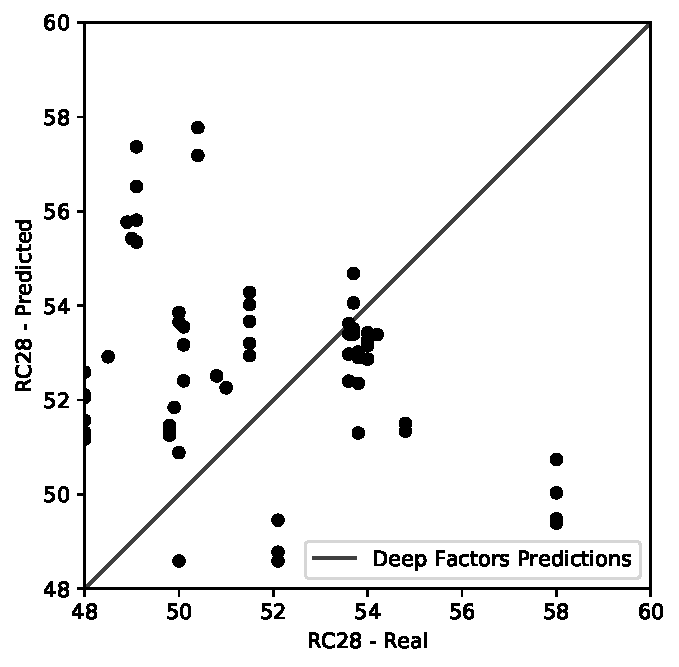
\includegraphics[height=0.3\textwidth]{/Users/thiagolira/Dropbox/Mestrado/Intercement/paper_img/qq_deep_factors.pdf} 
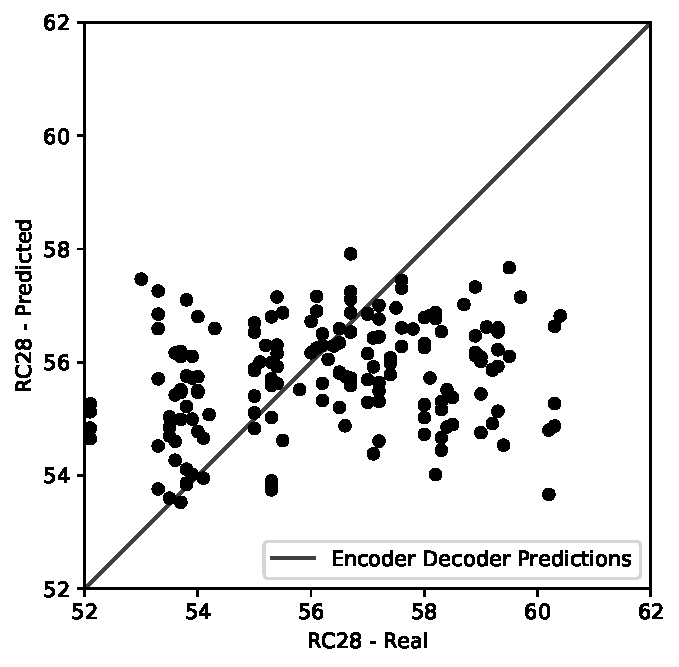
\includegraphics[height=0.3\textwidth]{/Users/thiagolira/Dropbox/Mestrado/Intercement/paper_img/qq_enc_dec.pdf} 
\end{center}

The Encoder-Decoder models seems to be able to best model the target distribution.

To evaluate the quality of the uncertainty measures, we shall use the .5 risk and .9 risk metrics. For each model 
we will compare the risks for the predictions of the next day, the next 3 days and the next 7 days. (The bigger the number the worse is the uncertainty).

\begin{center}
\begin{table}[H]
\caption{\label{tab:orgf7c5e45}
Table with risks for each timespan forecast}
\centering
\begin{tabular}{lrr}
\hline
Encoder Decoder & .5 risk & .9 risk\\
\hline
24h & 0.004 & 0.025\\
3d & 0.005 & 0.02\\
7d & 0.011 & 0.037\\
\hline
Deep Factors & .5 risk & .9 risk\\
\hline
24h & 0.001 & 0.036\\
3d & 0.009 & 0.031\\
7d & 0.023 & 0.027\\
\hline
Deep AR & .5 risk & .9 risk\\
\hline
24h & 0.009 & 0.004\\
3d & 0.018 & 0.008\\
7d & 0.044 & 0.016\\
\hline
\end{tabular}
\end{table}
\end{center}


As Table \ref{tab:orgf7c5e45} shows, the 3 models have good next-day predictions, with a low .5 risk. All risks increase as the forecast acts further in the future, as is expected.



\section{Conclusion}
\label{sec:org1323f05}

TO DO

\bibliographystyle{plain}
\bibliography{bibliografia}{}
\end{document}